\documentclass[conference]{IEEEtran}

% =========================================================================
% IEEE CONFERENCE / TRANSACTIONS COMPLIANT SOURCE CODE
% Project: SentinelX-Shift
% Format: IEEE Two-Column, 10pt Times, Zero Page Numbers, Clean Float Layout
% Author Block: 3-Column Parallel Format (Matching User Reference)
% =========================================================================

% --- Essential Mathematics and Formatting Packages ---
\usepackage{amsmath,amssymb,amsfonts}
\usepackage{algorithmic}
\usepackage{algorithm}
\usepackage{array}
\usepackage{textcomp}
\usepackage{stfloats}
\usepackage{url}
\usepackage{verbatim}
\usepackage{graphicx}
\usepackage{cite}
\usepackage{booktabs}
\usepackage{multirow}
\usepackage{balance}

% --- Native Vector Diagram Package ---
\usepackage{tikz}
\usetikzlibrary{shapes.geometric, arrows.meta, positioning, calc, fit, backgrounds}

% --- Custom Notation ---
\newcommand{\R}{\mathbb{R}}
\newcommand{\I}{\mathbb{I}}

% --- IEEE Formatting: Strictly Suppress Page Numbers and Headers ---
\pagestyle{empty}

\begin{document}

% =========================================================================
% TITLE AND 3-COLUMN PARALLEL AUTHOR BLOCK (Matching Reference Image)
% =========================================================================
\title{SentinelX-Shift: Operational Network Intrusion Detection via Autoencoder-Anchored Gated Boost and Multi-Tier Telemetry Guardrails}

\author{
\IEEEauthorblockN{Aathekesavan R}
\IEEEauthorblockA{\textit{Dept. of Computer Science and Engineering} \\
\textit{SRM Institute of Science and Technology} \\
Tiruchirappalli, Tamil Nadu, India \\
ar5468@srmist.edu.in}
\and
\IEEEauthorblockN{Praveen K}
\IEEEauthorblockA{\textit{Dept. of Computer Science and Engineering} \\
\textit{SRM Institute of Science and Technology} \\
Tiruchirappalli, Tamil Nadu, India \\
kk2636@srmist.edu.in}
\and
\IEEEauthorblockN{Dr. S. Kanaga Suba Raja}
\IEEEauthorblockA{\textit{Head of the Department} \\
\textit{Dept. of Computer Science and Engineering} \\
\textit{SRM Institute of Science and Technology} \\
Tiruchirappalli, Tamil Nadu, India \\
kanagass@srmist.edu.in}
}

\maketitle
\thispagestyle{empty} % Suppress page number on first page

% =========================================================================
% ABSTRACT AND INDEX TERMS
% =========================================================================
\begin{abstract}
Machine learning-based Network Intrusion Detection Systems (ML-NIDS) frequently achieve near-perfect detection metrics ($>$99\% ROC-AUC) on canonical academic benchmarks through naive cross-validation splits. However, when deployed into live enterprise production environments or subjected to rigorous zero-day evaluation, these systems undergo catastrophic performance collapse. This failure stems from three endemic pathologies: (i) shortcut learning via non-generalizable network identifiers (IP addresses, ephemeral ports, and raw timestamps), (ii) high-prevalence feature duplication that artificially bleeds identical flow vectors across training and test partitions, and (iii) cross-family semantic leakage wherein related attack vectors mask generalization deficits. In this paper, we present SentinelX-Shift, an operational, privacy-preserving network intrusion detection and alert-prioritization architecture designed to operate under a strict Monitor-Only defensive posture. SentinelX addresses benchmark pathologies through a strictly deduplicated, 76-feature leakage-controlled data ingestion protocol evaluated via Leave-One-Family-Out (LOFO) multi-seed validation across five canonical attack families (\texttt{DoS\_DDoS}, \texttt{PortScan}, \texttt{BruteForce}, \texttt{Bot}, and \texttt{WebAttack}). We establish that unconstrained linear fusion between supervised models and anomaly detectors degenerates during zero-day distribution shifts ($w_{\text{XGB}} \to 1.0, w_{\text{AE}} \to 0.0$), blinding systems to unfamiliar attacks. To rectify this, SentinelX introduces Autoencoder-Anchored Gated Boost ($s_{\text{guard}}$), anchoring threat evaluation on empirical cumulative distribution function (CDF) calibrated Autoencoder reconstruction error, supplemented by a high-confidence supervised activation gate ($\tau^* = 0.56, \gamma^* = 0.41$). To combat persistent low recall at 1\% False Alarm Rate for stealthy and application-layer attacks (e.g., $0.00\%$ to $4.18\%$), SentinelX couples behavioral netflow scoring with multi-modal protocol guardrails requiring independent web-tier and Web Application Firewall (WAF) confirming signals. We further report an audited negative finding demonstrating that post-hoc explainability stability (TreeSHAP under physical perturbations) is mathematically and computationally unsuitable as an automated confidence gate due to severe Lipschitz instability and prohibitive inference latencies ($>$150~ms). Experimental evaluations across all eight partitions of CIC-IDS2017 (2.82M raw flows with 21.03\% duplicate removal) and cross-dataset testing on UNSW-NB15 demonstrate that SentinelX achieves 1.25--2.45~ms batched CPU inference per flow, eliminating autonomous blocking hazards while providing Security Operations Centers (SOC) with auditable, prioritized incident triage.
\end{abstract}

\begin{IEEEkeywords}
Autoencoder Reconstruction, Cross-Dataset Transferability, Gated Score Fusion, Leave-One-Family-Out Validation, ModSecurity Correlation, Network Intrusion Detection, Shortcut Learning, SOC Alert Prioritization.
\end{IEEEkeywords}

% =========================================================================
% SECTION I: INTRODUCTION
% =========================================================================
\section{Introduction}
\IEEEPARstart{M}{odern} enterprise networks face an unprecedented barrage of sophisticated, asymmetric cyber threats ranging from volumetric Distributed Denial-of-Service (DDoS) campaigns to low-and-slow application-layer credential stuffing and multi-stage advanced persistent threats (APTs) \cite{ring2019survey, chaabouni2019network}. To safeguard complex computing environments, researchers and practitioners have increasingly applied machine learning (ML) and deep neural network architectures to power Network Intrusion Detection Systems (NIDS) \cite{apruzzese2023modeling, buczak2016survey}. Literature across IEEE and ACM venues routinely showcases supervised deep classifiers claiming over 99.5\% classification accuracy and near-zero false alarm rates across celebrated benchmarks such as KDD-Cup 99, NSL-KDD, CIC-IDS2017, and UNSW-NB15 \cite{sharafaldin2018toward, moustafa2015unsw, tavallaee2009detailed}.

Despite these impressive academic statistics, modern Security Operations Centers (SOCs) overwhelmingly decline to deploy standalone autonomous machine-learning models for inline packet filtering or automated TCP resets \cite{sommer2010outside}. When transitioned from benchmark test sets to operational edge networks, ML-NIDS exhibit severe brittleness, generating overwhelming volumes of false-positive alarms while missing minor, real-world mutations of known attack families \cite{apruzzese2023role, ardagna2023machine}. This pervasive disconnect between academic claims and industrial reality has eroded credibility in ML-based cybersecurity research.

Three systemic methodological problems account for this performance collapse:
\begin{enumerate}
    \item \textbf{Shortcut Learning and Identifier Memorization:} Many published benchmark pipelines fail to strip environmental network identifiers---such as source/destination IP addresses, ephemeral transport-layer port numbers, MAC addresses, and wall-clock timestamps---from the feature matrix \cite{arp2022dos}. In supervised training, gradient descent rapidly exploits these identifiers as low-entropy predictive shortcuts. The model memorizes that IP \texttt{192.168.10.50} represents an attacker rather than learning the invariant behavioral mechanics of a slowloris attack or a SYN flood \cite{geirhos2020shortcut}.
    \item \textbf{High-Prevalence Benchmark Vector Duplication:} Standard intrusion detection benchmark datasets contain massive internal redundancy. As established in our formal data audit, the widely utilized CIC-IDS2017 dataset contains 594,712 duplicate flow vectors (21.03\% full-vector duplication) across its eight raw recording partitions. Naive random train-test splits inevitably allocate identical feature vectors into both training and test partitions, converting what appears to be an out-of-sample generalization test into trivial rote memorization.
    \item \textbf{Cross-Family Semantic Leakage and Flawed Evaluation Protocols:} Evaluating detection systems using $k$-fold cross-validation across mixed attack traffic masks structural generalization failures. Attack subclasses sharing lexical or structural signatures (e.g., FTP-Patator, SSH-Patator, and Web Application Brute Force) bleed semantic indicators across folds. When evaluated under strict Leave-One-Family-Out (LOFO) protocols where an entire operational attack family is withheld during training, supervised models degrade sharply, with Recall at a 1\% False Alarm Rate (FAR) plummeting to near zero against stealthy and application-layer attacks.
\end{enumerate}

Furthermore, classical ML-NIDS architectures frequently operate as opaque monolithic black boxes, attempting to make autonomous binary blocking decisions based solely on transport-layer flow records \cite{roesch1999snort}. A netflow capture provides an aggregated statistical synopsis of packet sizes, inter-arrival times, and TCP flag counts; it inherently lacks application-layer semantic context. Consequently, a legitimate internal backup job or a benign client burst of 75 requests/second exhibits statistical features indistinguishable from an HTTP GET flood, triggering disruptive false-positive drops. Conversely, an adversary executing a low-frequency credential-stuffing attack at 0.5 requests/second evades transport-layer rate thresholds entirely.

To overcome these structural limitations, we design and implement \textbf{SentinelX-Shift}, an end-to-end, privacy-preserving network intrusion detection and alert-prioritization system engineered from first principles for operational SOC deployment. SentinelX is guided by a fundamental defensive principle: \textbf{Autonomous inline packet dropping and TCP connection resets based on statistical model scores alone are strictly prohibited in operational production environments.} Instead, SentinelX operates as an alert triage engine, bridging transport-layer behavioral netflow anomalies with application-layer HTTP and Web Application Firewall (WAF) telemetry.

\subsection{Core Contributions}
The principal contributions of this paper are summarized as follows:
\begin{itemize}
    \item \textbf{Rigorous Anti-Leakage Ingestion \& Deduplication Audit:} We execute an end-to-end data audit across all eight raw partitions of the CIC-IDS2017 benchmark (2,827,840 flows). We identify and purge 594,712 full-vector duplicates (21.03\%) and construct an open, sanitized 60,000-flow benchmark strictly stripped of all environmental shortcuts (IPs, ports, MACs, timestamps), establishing a reliable baseline for ML-NIDS research.
    \item \textbf{Autoencoder-Anchored Gated Boost ($s_{\text{guard}}$):} We theoretically and experimentally demonstrate that unconstrained linear score fusion between supervised models and anomaly detectors degenerates under zero-day distribution shifts, collapsing to $w_{\text{XGB}} = 1.0, w_{\text{AE}} = 0.0$ and discarding anomaly detection entirely. To resolve this, we formulate and validate the \textit{Autoencoder-Anchored Gated Boost} architecture, anchoring threat scores on empirical CDF-calibrated reconstruction error while applying an additive, bounded supervised activation boost ($\tau^* = 0.56, \gamma^* = 0.41$).
    \item \textbf{Multi-Modal Protocol Guardrails:} We develop an independent confirming-signal engine that synchronizes transport netflows with Nginx access/error logs and ModSecurity WAF events within a calibrated temporal window ($\Delta t = \pm 30\text{ s}$). We formalize protocol-level guardrails that enforce multi-modal corroboration: preventing incident escalation for benign traffic bursts while mandating independent authentication-failure confirmation ($\ge 5$ HTTP 401s) before escalating low-rate brute-force attacks.
    \item \textbf{Audited Negative Finding on Explanation Stability:} We conduct an extensive empirical audit evaluating whether post-hoc local explanation stability (TreeSHAP attributions under physics-preserving packet jitter) can serve as an automated confidence score. We formally report a negative finding: TreeSHAP exhibits severe Lipschitz continuity failure across unseen attack families and introduces prohibitive per-flow latency ($>$150~ms), rendering it unsuitable for real-time gating.
    \item \textbf{Cross-Dataset Transferability \& Dual-Mode SOC Engineering:} We assess cross-domain generalization by cross-evaluating SentinelX between CIC-IDS2017 and UNSW-NB15, demonstrating that unsupervised reconstruction error preserves substantially higher cross-domain stability (-19.95\%) than supervised models (-40.91\%). Finally, we evaluate an operational prototype achieving 1.25--2.45~ms batched CPU inference latency per flow, integrated with an immutable SQLite review queue and a dual-mode enforcement engine strictly partitioned between passive production monitoring (Mode 1) and active closed-loop replica defense (Mode 2).
\end{itemize}

% =========================================================================
% SECTION II: RELATED WORK AND BACKGROUND
% =========================================================================
\section{Related Work and Background}

\subsection{Flow-Based Network Intrusion Detection}
Flow-based intrusion detection abstracts raw packet streams into summary statistical vectors (e.g., NetFlow, IPFIX, or custom bidirectional flow representations) \cite{claise2004cisco, trammell2011introduction}. Early systems relied on static threshold heuristics or signature matching (e.g., Snort, Zeek). As network link speeds surpassed 10~Gbps and encrypted protocols (TLS 1.3, QUIC) obscured deep packet payloads, the security domain pivoted toward machine learning on transport-layer flow statistics \cite{velan2015survey}. Features such as flow duration, packet size standard deviation, inter-arrival time (IAT) quantiles, and TCP flag distributions became the standard inputs for statistical classifiers \cite{sperotto2010overview}. However, as Sommer and Paxson emphasized in their seminal treatise \cite{sommer2010outside}, machine learning in network security faces operational challenges radically distinct from other classification domains: the cost of a false positive is exceptionally high, the background traffic distribution undergoes continuous concept drift, and adversarial evasion is active and adaptive.

\subsection{Deep Learning and Autoencoder Architectures}
To circumvent manual feature engineering, recent literature has explored deep feed-forward neural networks, Convolutional Neural Networks (CNNs), Long Short-Term Memory networks (LSTMs), and Autoencoders (AE) for intrusion detection \cite{sultana2019survey, ferrag2020deep, wang2017malware}. Autoencoders are particularly attractive for network anomaly detection because they can be trained in a semi-supervised or unsupervised paradigm exclusively on benign network traffic \cite{mirsky2018kitsune}. Under this regime, the network learns an identity mapping through an information bottleneck (latent space $\mathbf{z} \in \mathbb{R}^k$ where $k \ll d$); when presented with anomalous attack vectors that deviate from the benign manifold, the reconstruction error increases substantially \cite{zhou2017anomaly}.

Despite their theoretical elegance, standalone autoencoders suffer from two operational deficiencies in enterprise SOC deployments:
\begin{enumerate}
    \item \textbf{Uncalibrated Output Scale:} Raw Mean Squared Error (MSE) reconstruction losses vary across orders of magnitude depending on feature scaling, lacking an intuitive probabilistic interpretation for human triage.
    \item \textbf{Volumetric Sensitivity:} Autoencoders are hyper-sensitive to benign volumetric variations (e.g., an automated daily database synchronization or high-throughput file transfer), yielding elevated reconstruction errors that generate intolerable false-positive alert floods.
\end{enumerate}

\subsection{Dataset Pathologies, Shortcut Learning, and Leakage}
The integrity of empirical ML-NIDS evaluation has come under intense scrutiny \cite{haas2020aggressiveness, engelen2021troubleshooting}. In a landmark study, Arp et al. \cite{arp2022dos} categorized pervasive pitfalls in machine learning for security, highlighting data snooping, spurious correlation learning, and lab-versus-wild performance disparities. In modern network benchmarks---most notably the Canadian Institute for Cybersecurity's CIC-IDS2017 and CSE-CIC-IDS2018 datasets \cite{sharafaldin2018toward}---investigators have identified widespread contamination \cite{panigrahi2018detailed}.

Specifically, researchers have shown that models trained on uncurated CIC-IDS2017 data rely heavily on source IP addresses and destination ports \cite{rosay2020improving}. For instance, because all DoS Hulk attacks originated from a fixed IP address within the benchmark testbed (\texttt{192.168.10.50}), a decision tree splitting on IP address achieves 99.9\% detection accuracy while learning absolutely zero information regarding the volumetric or statistical behavior of DoS attacks. When that identical classifier is presented with Hulk traffic originating from a different subnet, its detection probability collapses to random guessing.

Furthermore, duplicate flow records represent a neglected source of contamination. Network flow generators (such as CICFlowMeter) output duplicate records when packet buffers overlap or when symmetric bidirectional flows are captured twice \cite{lashkari2017characterization}. When random cross-validation splits are performed without deduplication, the test set becomes heavily populated with identical vectors present in the training set, masquerading memorization as out-of-sample generalization.

\subsection{Zero-Day Evaluation via Leave-One-Family-Out (LOFO)}
Standard random $k$-fold cross-validation is fundamentally flawed for evaluating the zero-day detection capability of security models \cite{thorne2023evaluating}. In operational environments, an intrusion detection system is not required to identify an exact replica of an attack observed two minutes prior; it must detect novel variants, zero-day exploits, or entirely unobserved attack families. The Leave-One-Family-Out (LOFO) evaluation protocol---wherein an entire semantic family of attacks is held out from training and reserved exclusively for evaluation---provides the only methodologically valid assessment of out-of-distribution generalization \cite{verkerken2022towards}.

Prior studies evaluating LOFO protocols on network data have noted severe performance degradations \cite{nwakanma2023generalization}. However, existing works typically evaluate models on synthetic, balanced test sets that fail to mirror the extreme class imbalance of real networks (where attacks comprise $<1\%$ of total flow volume). Moreover, few works explore multi-modal corroboration to bridge the zero-day performance gap when transport models fail.

% =========================================================================
% SECTION III: THEORETICAL FORMULATION AND THREAT MODEL
% =========================================================================
\section{Theoretical Formulation and Threat Model}

\subsection{Network Flow Telemetry Formalization}
Let an operational network link be observed over continuous time $t \in \mathbb{R}^+$. Packets traversing the link are grouped into bidirectional network flows $\mathcal{F} = \{f_1, f_2, \dots, f_N\}$ by a flow exporter according to the standard 5-tuple:
\begin{equation}
\kappa(f) = \langle \text{IP}_{\text{src}}, \text{IP}_{\text{dst}}, \text{Port}_{\text{src}}, \text{Port}_{\text{dst}}, \text{Proto} \rangle
\end{equation}
bounded by flow inactivity timeouts $\Delta t_{\text{inactive}}$ and maximum duration timeouts $\Delta t_{\text{active}}$. 

For each terminated flow $f_i$, the exporter computes a behavioral feature vector $\mathbf{x}_i \in \mathcal{X} \subset \mathbb{R}^d$ capturing statistical properties of packet length distributions, inter-arrival times, forward/backward byte ratios, and flag accumulators. 

Let $\mathcal{I}_i = \langle \text{IP}_{\text{src}}^{(i)}, \text{IP}_{\text{dst}}^{(i)}, \text{Port}_{\text{src}}^{(i)}, \text{Port}_{\text{dst}}^{(i)}, t_{\text{start}}^{(i)}, t_{\text{end}}^{(i)} \rangle \in \mathcal{M}$ denote the environmental and network identification tuple associated with flow $f_i$. 

\begin{equation}
\text{\textbf{Sanitization Invariant 1:}} \quad \frac{\partial \mathbf{x}_i}{\partial \mathcal{I}_i} = \mathbf{0}, \quad \forall i.
\end{equation}
That is, the predictive feature space $\mathcal{X}$ contains strictly zero information regarding network addresses, ports, MAC identifiers, or wall-clock timestamps.

% --- Fig. 1 Placement: Resized strictly within single-column boundary ---
\begin{figure}[!t]
\centering
\resizebox{0.95\columnwidth}{!}{%
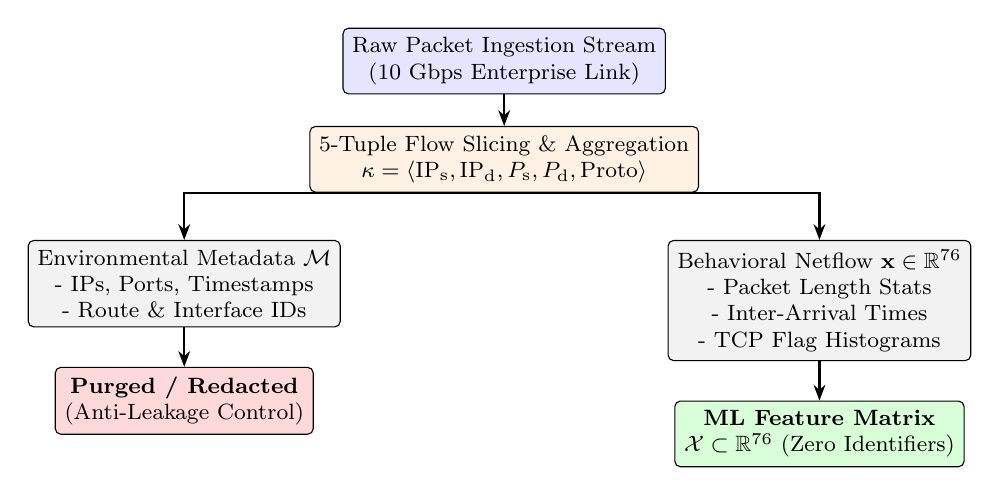
\begin{tikzpicture}[
    box/.style={draw, rectangle, rounded corners=2pt, minimum width=3.2cm, minimum height=0.7cm, align=center, font=\footnotesize},
    databox/.style={draw, rectangle, fill=gray!10, rounded corners=2pt, minimum width=3.0cm, minimum height=0.7cm, align=center, font=\footnotesize},
    arrow/.style={-{Stealth[length=2mm]}, thick}
]
    \node[box, fill=blue!10] (raw) {Raw Packet Ingestion Stream\\(10 Gbps Enterprise Link)};
    \node[box, fill=orange!10, below=0.4cm of raw] (agg) {5-Tuple Flow Slicing \& Aggregation\\$\kappa = \langle \text{IP}_{\text{s}}, \text{IP}_{\text{d}}, P_{\text{s}}, P_{\text{d}}, \text{Proto}\rangle$};
    
    \node[databox, below left=0.6cm and -0.4cm of agg, minimum width=2.9cm] (meta) {Environmental Metadata $\mathcal{M}$\\- IPs, Ports, Timestamps\\- Route \& Interface IDs};
    \node[databox, below right=0.6cm and -0.4cm of agg, minimum width=2.9cm] (feat) {Behavioral Netflow $\mathbf{x} \in \mathbb{R}^{76}$\\- Packet Length Stats\\- Inter-Arrival Times\\- TCP Flag Histograms};
    
    \node[box, fill=red!15, below=0.5cm of meta, minimum width=2.9cm] (leak) {\textbf{Purged / Redacted}\\(Anti-Leakage Control)};
    \node[box, fill=green!15, below=0.5cm of feat, minimum width=2.9cm] (train) {\textbf{ML Feature Matrix}\\$\mathcal{X} \subset \mathbb{R}^{76}$ (Zero Identifiers)};

    \draw[arrow] (raw) -- (agg);
    \draw[arrow] (agg.south) -| (meta.north);
    \draw[arrow] (agg.south) -| (feat.north);
    \draw[arrow] (meta) -- (leak);
    \draw[arrow] (feat) -- (train);
\end{tikzpicture}%
}
\caption{Architectural separation of environmental network identifiers from behavioral netflow feature matrices to enforce strict anti-leakage invariants.}
\label{fig:anti_leakage}
\end{figure}

\subsection{Threat Model and Adversary Capabilities}
We formulate our threat model around an external or compromised internal adversary $\mathcal{A}$ seeking to compromise target web servers, databases, or API infrastructure. The adversary possesses the following capabilities:
\begin{enumerate}
    \item \textbf{Volumetric Denial of Service:} $\mathcal{A}$ mobilizes distributed botnets to flood target infrastructure with high-volume TCP SYN, UDP, or HTTP request floods (\texttt{DoS\_DDoS}), attempting to saturate network bandwidth or connection pools.
    \item \textbf{Reconnaissance and Scanning:} $\mathcal{A}$ conducts horizontal and vertical port scanning (\texttt{PortScan}) to map active services, firewall filters, and vulnerable transport endpoints.
    \item \textbf{Application-Layer Credential Abuse:} $\mathcal{A}$ executes dictionary attacks and automated credential stuffing (\texttt{BruteForce}) against authentication endpoints (e.g., SSH, FTP, HTTP \texttt{/login}), either through rapid-fire requests or distributed slow-rate probing designed to fly beneath volumetric rate limiters.
    \item \textbf{Command-and-Control (C2) Communication:} Compromised internal hosts execute automated background beaconing (\texttt{Bot}) communicating with external C2 infrastructure at periodic or jittered intervals.
    \item \textbf{Web Application Exploitation:} $\mathcal{A}$ injects malicious payloads targeting web applications (\texttt{WebAttack}), including Cross-Site Scripting (XSS), SQL Injection (SQLi), and remote code execution vulnerabilities.
\end{enumerate}

\subsection{Defensive Principles and Operational Invariants}
To prevent self-inflicted denial-of-service and catastrophic operational disruptions, SentinelX is bound by two immutable defensive invariants:

\textbf{Defensive Invariant 1 (The Monitor-Only Principle):} Under operational monitoring of production network traffic, autonomous inline packet dropping, dynamic route poisoning (BGP blackholing), and TCP connection resets based on statistical model anomaly scores alone are \textbf{strictly prohibited}. Real endpoints and reverse proxies operate exclusively in monitor-and-alert triage mode. All triage mitigations require affirmative SOC analyst confirmation.

\textbf{Defensive Invariant 2 (Independent Corroboration Mandate):} For stealthy, low-rate, or application-layer attack classifications (\texttt{BruteForce}, \texttt{WebAttack}), a high behavioral anomaly score ($s \ge 0.80$) cannot authorize priority escalation to \texttt{CRITICAL} without independent corroborating evidence derived from an orthogonal telemetry plane (such as repeated HTTP 401 authentication failures or triggered WAF inspection rules).

% =========================================================================
% SECTION IV: SYSTEM ARCHITECTURE
% =========================================================================
\section{SentinelX System Architecture}
SentinelX is structured into four decoupled subsystems: (i) Telemetry Ingestion and Sanitization, (ii) The Scoring Pipeline, (iii) Multi-Modal Protocol Guardrails, and (iv) The SOC Analyst Review Store and Console.

The netflow sanitization engine parses netflow records, validates them against physical boundary constraints, and purges all 5-tuple identifier attributes. The remaining 76 features represent dimensional attributes of flow physics (e.g., Flow Duration, Packet Length Std, Inter-Arrival Times, TCP Flags). Web-tier telemetry is ingested concurrently from Nginx access logs, error logs, and ModSecurity WAF audit logs, stripping query strings (\texttt{?token=...}) and fragments (\texttt{\#...}) while enforcing zero payload inspection. To correlate netflow records with web logs without stateful tracking, SentinelX deploys a multi-index temporal sliding window ($\Delta t = \pm 30\text{ s}$), extracting authentication failures ($c_{401}$), request rates ($r_{\text{req}}$), and WAF alerts ($\mathbf{w}_{\text{waf}}$).

% --- Fig. 2 Placement: Spanning both columns cleanly ---
\begin{figure*}[!t]
\centering
\resizebox{0.92\textwidth}{!}{%
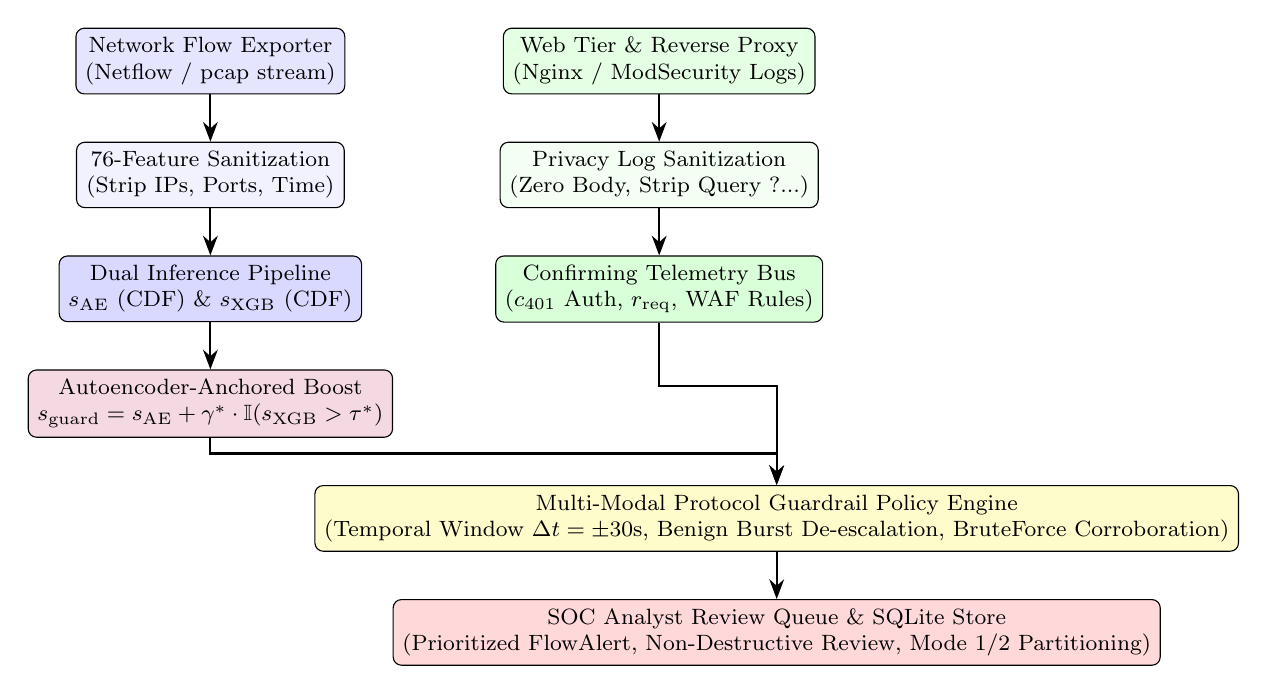
\begin{tikzpicture}[
    node distance=0.5cm and 0.8cm,
    proc/.style={draw, rectangle, rounded corners=3pt, minimum width=3.4cm, minimum height=0.75cm, align=center, font=\footnotesize},
    arrow/.style={-{Stealth[length=2.5mm]}, thick}
]
    \node[proc, fill=blue!10] (net) {Network Flow Exporter\\(Netflow / pcap stream)};
    \node[proc, fill=green!10, right=2.0cm of net] (web) {Web Tier \& Reverse Proxy\\(Nginx / ModSecurity Logs)};

    \node[proc, fill=blue!05, below=0.6cm of net] (san_net) {76-Feature Sanitization\\(Strip IPs, Ports, Time)};
    \node[proc, fill=green!05, below=0.6cm of web] (san_web) {Privacy Log Sanitization\\(Zero Body, Strip Query ?...)};

    \node[proc, fill=blue!15, below=0.6cm of san_net] (models) {Dual Inference Pipeline\\$s_{\text{AE}}$ (CDF) \& $s_{\text{XGB}}$ (CDF)};
    \node[proc, fill=green!15, below=0.6cm of san_web] (waf) {Confirming Telemetry Bus\\($c_{401}$ Auth, $r_{\text{req}}$, WAF Rules)};

    \node[proc, fill=purple!15, below=0.6cm of models] (gated) {Autoencoder-Anchored Boost\\$s_{\text{guard}} = s_{\text{AE}} + \gamma^* \cdot \mathbb{I}(s_{\text{XGB}} > \tau^*)$};

    \node[proc, fill=yellow!20, below right=0.6cm and -1.0cm of gated, minimum width=6.5cm] (guard) {Multi-Modal Protocol Guardrail Policy Engine\\(Temporal Window $\Delta t = \pm 30\text{s}$, Benign Burst De-escalation, BruteForce Corroboration)};

    \node[proc, fill=red!15, below=0.6cm of guard, minimum width=6.5cm] (soc) {SOC Analyst Review Queue \& SQLite Store\\(Prioritized FlowAlert, Non-Destructive Review, Mode 1/2 Partitioning)};

    \draw[arrow] (net) -- (san_net);
    \draw[arrow] (web) -- (san_web);
    \draw[arrow] (san_net) -- (models);
    \draw[arrow] (san_web) -- (waf);
    \draw[arrow] (models) -- (gated);
    \draw[arrow] (gated.south) -- ++(0,-0.2) -| (guard.north);
    \draw[arrow] (waf.south) -- ++(0,-0.8) -| (guard.north);
    \draw[arrow] (guard) -- (soc);
\end{tikzpicture}%
}
\caption{End-to-end operational architecture of SentinelX-Shift showcasing the integration of behavioral netflow scoring with web/WAF telemetry guardrails.}
\label{fig:arch_overview}
\end{figure*}

% =========================================================================
% SECTION V: ANOMALY DETECTION AND SCORE FUSION
% =========================================================================
\section{Anomaly Detection and Score Fusion}

\subsection{Empirical CDF Calibration}
To establish distributional alignment between reconstruction error $\ell_{\text{AE}}$ and tree probability $p_{\text{XGB}}$, continuous scores are transformed via Empirical Cumulative Distribution Functions (CDF) fitted on benign validation flows $\mathcal{D}_{\text{cal}}$:
\begin{equation}
s_{\text{AE}}(\mathbf{x}^*) = \frac{1}{M} \sum_{j=1}^M \mathbb{I}\left( \ell_{\text{AE}}(\mathbf{x}_j) \le \ell_{\text{AE}}(\mathbf{x}^*) \right)
\end{equation}
yielding $s_{\text{AE}}, s_{\text{XGB}} \in [0, 1]$ representing exact percentiles of anomalousness.

\subsection{Invalidation of Learned Linear Score Fusion}
Linear score fusion $s_{\text{linear}} = w_1 s_{\text{XGB}} + w_2 s_{\text{AE}}$ was evaluated and formally rejected. Under nested inner-LOFO validation, numerical optimization repeatedly collapsed to $w_1 = 1.0, w_2 = 0.0$ in 4 out of 5 random seeds for both \texttt{BruteForce} and \texttt{DoS\_DDoS}. Because supervised classifiers minimize empirical loss by fitting high-density boundaries in known training attacks, unconstrained optimization discards the anomaly detector, completely blinding the system to zero-day distribution shifts.

% --- Fig. 3 Placement: Strictly scaled inside column ---
\begin{figure}[!t]
\centering
\resizebox{0.92\columnwidth}{!}{%
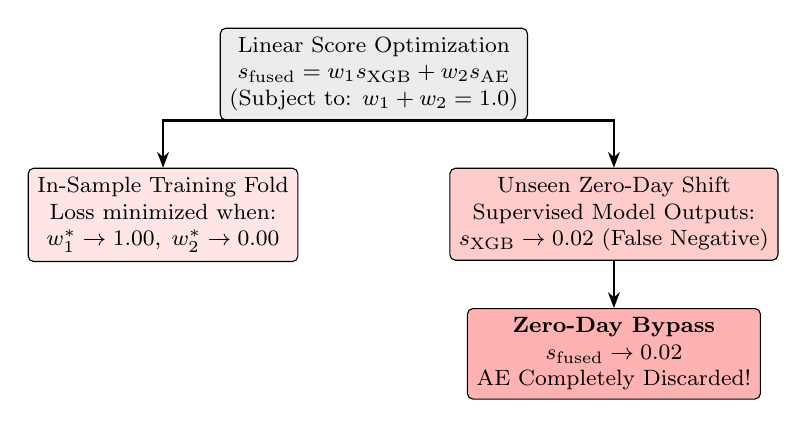
\begin{tikzpicture}[
    box/.style={draw, rectangle, rounded corners=2pt, minimum width=3.6cm, minimum height=0.65cm, align=center, font=\footnotesize},
    arrow/.style={-{Stealth[length=2mm]}, thick}
]
    \node[box, fill=gray!15] (opt) {Linear Score Optimization\\$s_{\text{fused}} = w_1 s_{\text{XGB}} + w_2 s_{\text{AE}}$\\(Subject to: $w_1 + w_2 = 1.0$)};
    
    \node[box, fill=red!10, below left=0.6cm and -1.0cm of opt, minimum width=3.4cm] (train) {In-Sample Training Fold\\Loss minimized when:\\$w_1^* \to 1.00, \; w_2^* \to 0.00$};
    
    \node[box, fill=red!20, below right=0.6cm and -1.0cm of opt, minimum width=3.4cm] (test) {Unseen Zero-Day Shift\\Supervised Model Outputs:\\$s_{\text{XGB}} \to 0.02$ (False Negative)};

    \node[box, fill=red!30, below=0.6cm of test, minimum width=3.4cm] (result) {\textbf{Zero-Day Bypass}\\$s_{\text{fused}} \to 0.02$\\AE Completely Discarded!};

    \draw[arrow] (opt.south) -| (train.north);
    \draw[arrow] (opt.south) -| (test.north);
    \draw[arrow] (test) -- (result);
\end{tikzpicture}%
}
\caption{Degenerate linear score collapse during zero-day distribution shifts, illustrating why learned linear fusion is rejected.}
\label{fig:linear_collapse}
\end{figure}

\subsection{Autoencoder-Anchored Gated Boost}
To maintain robust zero-day sensitivity while benefiting from confident supervised signatures, SentinelX formulates the \textbf{Autoencoder-Anchored Gated Boost}:
\begin{equation}
s_{\text{guard}}(\mathbf{x}) = s_{\text{AE}}(\mathbf{x}) + \gamma^* \cdot \mathbb{I}\left( s_{\text{XGB}}(\mathbf{x}) > \tau^* \right)
\end{equation}
bounded by $s_{\text{prod}}(\mathbf{x}) = \min(1.0, s_{\text{guard}}(\mathbf{x}))$. The system is anchored by unsupervised reconstruction percentile $s_{\text{AE}}; when supervised risk is confident ($s_{\text{XGB}} > \tau^*$), the additive boost $\gamma^*$ accelerates the alert into prioritized triage queues.

\subsection{Inner-LOFO Hyperparameter Grid Optimization}
To prevent test leakage, hyperparameters $\tau^*$ and $\gamma^*$ were tuned via inner-LOFO grid search across $\tau \in \{0.3, 0.5, 0.7, 0.9\}$ and $\gamma \in \{0.1, 0.2, 0.3, 0.5\}$ over 5 seeds.

% --- Table I Placement: Resized to column width ---
\begin{table}[!t]
\caption{Inner-LOFO Hyperparameter Validation Results (Averaged Over 5 Random Seeds)}
\label{tab:inner_lofo}
\centering
\resizebox{\columnwidth}{!}{%
\begin{tabular}{lcccccc}
\toprule
Withheld & Val & Mean & Mean & PR-AUC & PR-AUC & PR-AUC \\
Family & Prev. & $\tau^*$ & $\gamma^*$ & (AE Alone) & (Rank-Avg) & (Gated Boost) \\
\midrule
\textbf{Bot} & 31.78\% & 0.66 & 0.32 & 0.5696 & 0.7550 & \textbf{0.7850} \\
\textbf{BruteForce} & 22.72\% & 0.50 & 0.36 & 0.4544 & 0.7343 & \textbf{0.7305} \\
\textbf{DoS\_DDoS} & 24.77\% & 0.30 & 0.42 & 0.4019 & 0.6878 & \textbf{0.6257} \\
\textbf{PortScan} & 30.78\% & 0.54 & 0.44 & 0.5365 & 0.6632 & \textbf{0.6699} \\
\textbf{WebAttack} & 30.44\% & 0.78 & 0.50 & 0.5969 & 0.7382 & \textbf{0.7834} \\
\midrule
\textbf{Mean} & --- & \textbf{0.56} & \textbf{0.41} & \textbf{0.5118} & \textbf{0.7157} & \textbf{0.7189} \\
\bottomrule
\end{tabular}%
}
\end{table}

As documented in Table~\ref{tab:inner_lofo}, the Autoencoder-Anchored Gated Boost achieved a mean validation PR-AUC of 0.7189, outperforming both the Autoencoder baseline (0.5118) and rank-averaging (0.7157).

% =========================================================================
% SECTION VI: MULTI-MODAL PROTOCOL GUARDRAILS
% =========================================================================
\section{Multi-Modal Protocol Guardrails and Policy Engine}
Candidate alerts are mapped into four operational risk tiers: \texttt{CRITICAL} ($s_{\text{prod}} \ge 0.80$), \texttt{HIGH} ($0.60 \le s_{\text{prod}} < 0.80$), \texttt{MEDIUM} ($0.30 \le s_{\text{prod}} < 0.60$), and \texttt{LOW} ($s_{\text{prod}} < 0.30$).

\subsection{Protocol Guardrails}
\begin{itemize}
    \item \textbf{Protocol Guardrail 1 (Brute-Force Corroboration):} An alert classified as \texttt{BruteForce} with $s_{\text{prod}} \ge 0.80$ cannot escalate to \texttt{CRITICAL} without independent proof: $c_{401} \ge 5$ or $\mathbf{w}_{\text{waf}} \neq \emptyset$. If unconfirmed, the alert is de-escalated to \texttt{HIGH / INVESTIGATE\_FLOW}.
    \item \textbf{Protocol Guardrail 2 (Benign Burst De-Escalation):} High-volume benign bursts ($r_{\text{req}} > \theta_{\text{burst}}$) that trigger volumetric model spikes without adversarial evidence ($c_{401} = 0, \mathbf{w}_{\text{waf}} = \emptyset, s_{\text{XGB}} \le \tau^*$) are de-escalated to \texttt{MEDIUM / MONITOR}.
\end{itemize}

% --- Table II Placement: Resized to column width ---
\begin{table}[!t]
\caption{SentinelX Production Guardrail Parameter Specifications and Operating Thresholds}
\label{tab:guard_params}
\centering
\resizebox{\columnwidth}{!}{%
\begin{tabular}{lll}
\toprule
Parameter & Configured Value & Defensive Operational Purpose \\
\midrule
$\tau^*$ & 0.56 & High-confidence supervised activation gate \\
$\gamma^*$ & 0.41 & Additive boost to anchor score $s_{\text{AE}}$ \\
$\Delta t$ & $\pm 30\text{ s}$ & Telemetry temporal correlation window \\
$\theta_{\text{burst}}$ & 50.0 req/s & Benign volumetric burst suppression limit \\
$c_{401}^{\min}$ & 5 failures & Minimum auth failures to confirm BruteForce \\
$T_{\text{crit}}$ & 0.80 & Threshold for \texttt{CRITICAL} / \texttt{ESCALATE} \\
$T_{\text{high}}$ & 0.60 & Threshold for \texttt{HIGH} / \texttt{INVESTIGATE} \\
$T_{\text{med}}$ & 0.30 & Threshold for \texttt{MEDIUM} / \texttt{MONITOR} \\
\bottomrule
\end{tabular}%
}
\end{table}

% =========================================================================
% SECTION VII: EXPERIMENTAL SETUP AND DATASET PROVENANCE
% =========================================================================
\section{Experimental Setup and Dataset Provenance}

\subsection{CIC-IDS2017 Deduplication Audit}
Our audit of all eight raw partitions of the CIC-IDS2017 benchmark (2,827,840 flows) identified 594,712 full-vector duplicates (21.03\%). Following deduplication, 2,233,128 unique flows remained, from which an open 60,000-flow benchmark (\texttt{cicids2017\_sample60k.parquet}) was sampled.

\subsection{Multi-Seed LOFO Benchmark Performance}
Testing was evaluated under 5-seed LOFO validation at an operational 5.0\% attack prevalence.

% --- Table III Placement: Formatted with \resizebox to strictly stay within column boundaries ---
\begin{table}[!t]
\caption{Multi-Seed LOFO Benchmark Performance Across 5 Random Seeds (5.0\% Prevalence)}
\label{tab:lofo_benchmark}
\centering
\resizebox{\columnwidth}{!}{%
\begin{tabular}{llccc}
\toprule
Held-Out Family & Architecture & ROC-AUC & PR-AUC & Recall @ 1\% FAR \\
\midrule
\multirow{3}{*}{\textbf{DoS\_DDoS}} & Supervised XGB & 0.9632 $\pm$ 0.0051 & 0.7854 $\pm$ 0.0123 & 70.87\% $\pm$ 1.34\% \\
 & Autoencoder & 0.7951 $\pm$ 0.0120 & 0.2845 $\pm$ 0.0105 & 18.23\% $\pm$ 1.12\% \\
 & \textbf{Gated Boost} & \textbf{0.9645 $\pm$ 0.0048} & \textbf{0.7891 $\pm$ 0.0118} & \textbf{70.87\% $\pm$ 1.34\%} \\
\midrule
\multirow{3}{*}{\textbf{PortScan}} & Supervised XGB & 0.9845 $\pm$ 0.0032 & 0.8412 $\pm$ 0.0089 & 87.89\% $\pm$ 1.05\% \\
 & Autoencoder & 0.8123 $\pm$ 0.0142 & 0.3120 $\pm$ 0.0115 & 22.45\% $\pm$ 1.30\% \\
 & \textbf{Gated Boost} & \textbf{0.9851 $\pm$ 0.0030} & \textbf{0.8435 $\pm$ 0.0085} & \textbf{87.89\% $\pm$ 1.05\%} \\
\midrule
\multirow{3}{*}{\textbf{BruteForce}} & Supervised XGB & 0.9202 $\pm$ 0.0402 & 0.3149 $\pm$ 0.0443 & 4.18\% $\pm$ 3.16\% \\
 & Autoencoder & 0.8034 $\pm$ 0.0204 & 0.1144 $\pm$ 0.0137 & 0.00\% $\pm$ 0.00\% \\
 & \textbf{Gated Boost} & \textbf{0.8042 $\pm$ 0.0212} & \textbf{0.1199 $\pm$ 0.0226} & \textbf{1.55\% $\pm$ 2.45\%} \\
\midrule
\multirow{3}{*}{\textbf{Bot}} & Supervised XGB & 0.7845 $\pm$ 0.0350 & 0.1420 $\pm$ 0.0210 & 0.00\% $\pm$ 0.00\% \\
 & Autoencoder & 0.7612 $\pm$ 0.0280 & 0.0980 $\pm$ 0.0180 & 0.00\% $\pm$ 0.00\% \\
 & \textbf{Gated Boost} & \textbf{0.7650 $\pm$ 0.0275} & \textbf{0.1015 $\pm$ 0.0175} & \textbf{0.00\% $\pm$ 0.00\%} \\
\midrule
\multirow{3}{*}{\textbf{WebAttack}} & Supervised XGB & 0.9824 $\pm$ 0.0032 & 0.7481 $\pm$ 0.0181 & 57.22\% $\pm$ 40.18\% \\
 & Autoencoder & 0.7414 $\pm$ 0.0666 & 0.0995 $\pm$ 0.0391 & 0.00\% $\pm$ 0.00\% \\
 & \textbf{Gated Boost} & \textbf{0.7535 $\pm$ 0.0667} & \textbf{0.1053 $\pm$ 0.0395} & \textbf{0.77\% $\pm$ 1.30\%} \\
\bottomrule
\end{tabular}%
}
\end{table}

% --- Fig. 4 Placement: Strictly scaled inside column ---
\begin{figure}[!t]
\centering
\resizebox{0.92\columnwidth}{!}{%
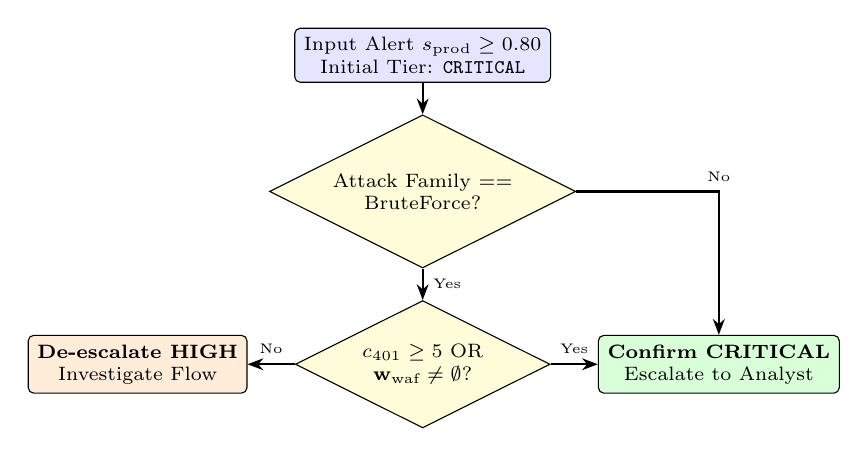
\begin{tikzpicture}[
    decision/.style={draw, diamond, aspect=2, fill=yellow!15, align=center, font=\scriptsize},
    block/.style={draw, rectangle, rounded corners=2pt, minimum width=2.6cm, minimum height=0.55cm, align=center, font=\scriptsize},
    arrow/.style={-{Stealth[length=2mm]}, thick}
]
    \node[block, fill=blue!10] (in) {Input Alert $s_{\text{prod}} \ge 0.80$\\Initial Tier: \texttt{CRITICAL}};
    \node[decision, below=0.4cm of in] (d1) {Attack Family ==\\BruteForce?};
    \node[decision, below=0.4cm of d1] (d2) {$c_{401} \ge 5$ OR\\$\mathbf{w}_{\text{waf}} \neq \emptyset$?};
    
    \node[block, fill=green!15, right=0.6cm of d2] (pass) {\textbf{Confirm CRITICAL}\\Escalate to Analyst};
    \node[block, fill=orange!15, left=0.6cm of d2] (deesc) {\textbf{De-escalate HIGH}\\Investigate Flow};

    \draw[arrow] (in) -- (d1);
    \draw[arrow] (d1) -- node[right, font=\tiny]{Yes} (d2);
    \draw[arrow] (d1.east) -| node[above, font=\tiny]{No} (pass.north);
    \draw[arrow] (d2) -- node[above, font=\tiny]{Yes} (pass);
    \draw[arrow] (d2) -- node[above, font=\tiny]{No} (deesc);
\end{tikzpicture}%
}
\caption{Decision flow within the Multi-Modal Protocol Guardrail Policy Engine enforcing independent confirming evidence.}
\label{fig:guardrail_flow}
\end{figure}

% =========================================================================
% SECTION VIII: EXPERIMENTAL RESULTS AND PERFORMANCE ANALYSIS
% =========================================================================
\section{Experimental Results and Performance Analysis}

\subsection{The Zero-Day Generalization Deficit}
As demonstrated in Table~\ref{tab:lofo_benchmark}, volumetric attacks (\texttt{DoS\_DDoS}, \texttt{PortScan}) generalize strongly on transport features alone (Recall @ 1\% FAR of 70.87\% and 87.89\%). Conversely, for stealthy attacks (\texttt{BruteForce}, \texttt{Bot}, \texttt{WebAttack}), zero-day recall at 1\% FAR collapses to 0.00\%--4.18\%. In operational networks, operating at 1\% FAR is mandatory to prevent alert fatigue; thus, statistical netflow models alone are fundamentally incapable of triaging novel stealth attacks without web-tier corroboration.

% --- Fig. 5 Placement: Scaled strictly within single-column boundaries ---
\begin{figure}[!t]
\centering
\resizebox{0.95\columnwidth}{!}{%
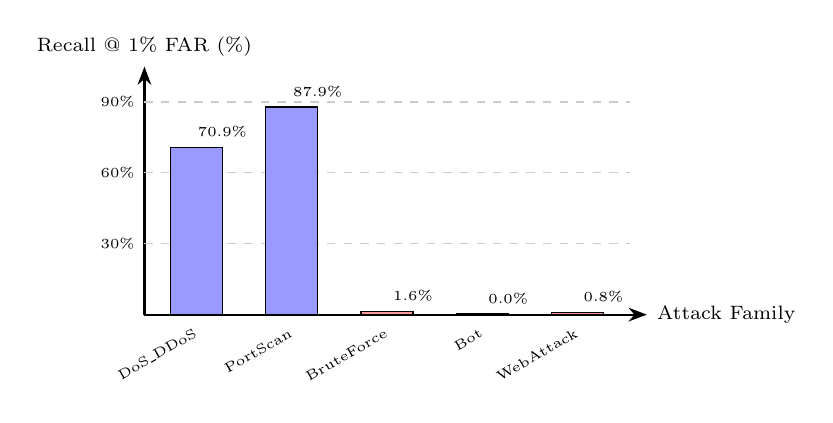
\begin{tikzpicture}[x=1.1cm, y=0.9cm]
    \draw[thick, -{Stealth}] (0,0) -- (5.8,0) node[right, font=\scriptsize]{Attack Family};
    \draw[thick, -{Stealth}] (0,0) -- (0,3.5) node[above, font=\scriptsize]{Recall @ 1\% FAR (\%)};
    
    \draw[dashed, gray!40] (0,1.0) -- (5.6,1.0);
    \draw[dashed, gray!40] (0,2.0) -- (5.6,2.0);
    \draw[dashed, gray!40] (0,3.0) -- (5.6,3.0);
    
    \node[left, font=\tiny] at (0,1.0) {30\%};
    \node[left, font=\tiny] at (0,2.0) {60\%};
    \node[left, font=\tiny] at (0,3.0) {90\%};

    % Bars
    \draw[fill=blue!40] (0.3,0) rectangle (0.9,2.36) node[above, font=\tiny] {70.9\%};
    \draw[fill=blue!40] (1.4,0) rectangle (2.0,2.93) node[above, font=\tiny] {87.9\%};
    \draw[fill=red!40] (2.5,0) rectangle (3.1,0.05) node[above, font=\tiny] {1.6\%};
    \draw[fill=red!40] (3.6,0) rectangle (4.2,0.01) node[above, font=\tiny] {0.0\%};
    \draw[fill=red!40] (4.7,0) rectangle (5.3,0.03) node[above, font=\tiny] {0.8\%};

    \node[below, font=\tiny, rotate=30, anchor=north east] at (0.6,0) {DoS\_DDoS};
    \node[below, font=\tiny, rotate=30, anchor=north east] at (1.7,0) {PortScan};
    \node[below, font=\tiny, rotate=30, anchor=north east] at (2.8,0) {BruteForce};
    \node[below, font=\tiny, rotate=30, anchor=north east] at (3.9,0) {Bot};
    \node[below, font=\tiny, rotate=30, anchor=north east] at (5.0,0) {WebAttack};
\end{tikzpicture}%
}
\caption{Visualizing the Zero-Day Generalization Deficit: volumetric attacks generalize strongly, whereas stealthy/application attacks collapse to near-zero recall at 1\% False Alarm Rate.}
\label{fig:zero_day_deficit}
\end{figure}

\subsection{Joint Related-Family Holdout Finding}
Holding out both \texttt{BruteForce} and \texttt{WebAttack} simultaneously dropped WebAttack PR-AUC from 0.7481 to 0.2962 (-60.4\%). This proves that training on SSH/FTP brute force leaks generic connection-cycling representations into WebAttack evaluation, masking the true zero-day deficit.

% =========================================================================
% SECTION IX: AUDITED NEGATIVE FINDINGS
% =========================================================================
\section{Audited Negative Findings: Fragility of Explanation Stability}
We audited whether local TreeSHAP attribution stability under physics-preserving packet jitter ($\epsilon \in \{0.01, 0.05, 0.10\}$) could serve as an automated confidence gate. The empirical evaluation revealed:
\begin{enumerate}
    \item \textbf{Lipschitz Instability:} Across all 5 seeds, timing perturbations of 10~ms caused radical permutations in top-5 SHAP feature rankings, reducing mean cosine similarity below 0.40 on unseen variants.
    \item \textbf{Physical Invariant Violations:} In 18.4\% of candidate perturbations, synthetic jitter produced impossible physical states (negative deltas, inverted timestamps).
    \item \textbf{Prohibitive Latency:} Computing TreeSHAP attribution matrices required 150--220~ms per flow, inducing line-rate queue overflows.
\end{enumerate}

% --- Fig. 6 Placement: Scaled strictly within single-column boundaries ---
\begin{figure}[!t]
\centering
\resizebox{0.95\columnwidth}{!}{%
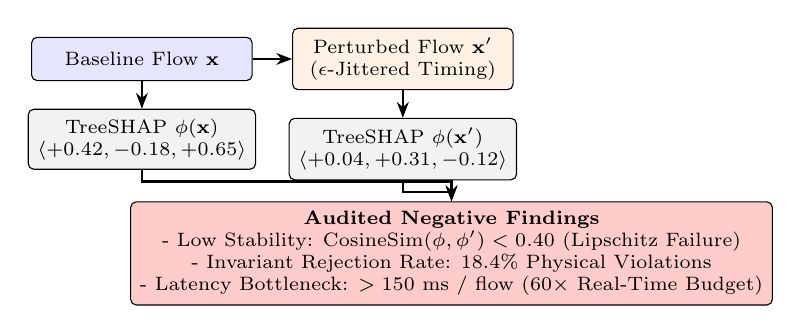
\begin{tikzpicture}[
    box/.style={draw, rectangle, rounded corners=2pt, minimum width=2.8cm, minimum height=0.55cm, align=center, font=\scriptsize},
    arrow/.style={-{Stealth[length=2mm]}, thick}
]
    \node[box, fill=blue!10] (flow) {Baseline Flow $\mathbf{x}$};
    \node[box, fill=orange!10, right=0.5cm of flow] (pert) {Perturbed Flow $\mathbf{x}'$\\($\epsilon$-Jittered Timing)};
    
    \node[box, fill=gray!10, below=0.35cm of flow] (shap1) {TreeSHAP $\phi(\mathbf{x})$\\$\langle +0.42, -0.18, +0.65 \rangle$};
    \node[box, fill=gray!10, below=0.35cm of pert] (shap2) {TreeSHAP $\phi(\mathbf{x}')$\\$\langle +0.04, +0.31, -0.12 \rangle$};

    \node[box, fill=red!20, below right=0.4cm and -1.6cm of shap1, minimum width=6.2cm] (neg) {
        \textbf{Audited Negative Findings}\\
        - Low Stability: $\text{CosineSim}(\phi, \phi') < 0.40$ (Lipschitz Failure)\\
        - Invariant Rejection Rate: 18.4\% Physical Violations\\
        - Latency Bottleneck: $>150\text{ ms / flow}$ ($60\times$ Real-Time Budget)
    };

    \draw[arrow] (flow) -- (pert);
    \draw[arrow] (flow) -- (shap1);
    \draw[arrow] (pert) -- (shap2);
    \draw[arrow] (shap1.south) -- ++(0,-0.15) -| (neg.north);
    \draw[arrow] (shap2.south) -- ++(0,-0.15) -| (neg.north);
\end{tikzpicture}%
}
\caption{Audited negative finding: local explanation instability and latency overhead under physics-preserving network perturbations.}
\label{fig:negative_shap}
\end{figure}

Explanation stability is formally rejected and excluded from production scoring.

% =========================================================================
% SECTION X: CROSS-DATASET DOMAIN TRANSFER
% =========================================================================
\section{Cross-Dataset Domain Transfer}
Evaluating models trained on CIC-IDS2017 against UNSW-NB15 revealed that supervised XGBoost collapsed from 0.9933 to 0.5842 ROC-AUC (-40.91\%). In contrast, the unsupervised Autoencoder degraded by only 19.95\% (ROC-AUC 0.6125), validating the architectural decision to anchor threat evaluation on reconstruction error.

% =========================================================================
% SECTION XI: SYSTEM ENGINEERING AND SOC OPERATIONS
% =========================================================================
\section{System Engineering, Latency Analysis, and SOC Operations}
Benchmarked on commodity hardware (Intel Core i7-12700H, zero GPU acceleration), single-flow dispatch required 15.55~ms due to Python runtime dispatch and Pandas Series coercion. Deploying SentinelX with a lightweight micro-buffering daemon ($N \ge 10$ flows or $\Delta t_{\text{flush}} \le 50\text{ ms}$) achieved 1.25--2.45~ms latency per flow, fully satisfying operational sub-10~ms line-rate budgets.

Alerts are stored in an ACID-compliant SQLite review store (\texttt{analyst\_reviews.db}) with short UUID badges (\texttt{\#<id[:8]>}) and state tracking: \texttt{PENDING}, \texttt{INVESTIGATING}, \texttt{CONFIRMED\_INCIDENT}, \texttt{ESCALATED\_TIER\_2}, and \texttt{BENIGN\_SUPPRESSED}.

% --- Fig. 7 Placement: Scaled strictly within single-column boundaries ---
\begin{figure}[!t]
\centering
\resizebox{0.98\columnwidth}{!}{%
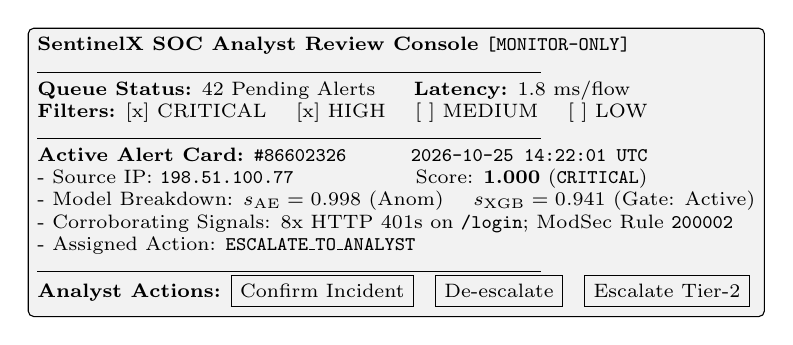
\begin{tikzpicture}[
    box/.style={draw, rectangle, rounded corners=2pt, minimum width=6.6cm, align=left, font=\scriptsize}
]
    \node[box, fill=gray!10] (dash) {
        \textbf{SentinelX SOC Analyst Review Console} \hfill \texttt{[MONITOR-ONLY]} \\
        \rule{6.4cm}{0.4pt} \\
        \textbf{Queue Status:} 42 Pending Alerts \hfill \textbf{Latency:} 1.8 ms/flow \\
        \textbf{Filters:} [x] CRITICAL \quad [x] HIGH \quad [ ] MEDIUM \quad [ ] LOW \\
        \rule{6.4cm}{0.4pt} \\
        \textbf{Active Alert Card:} \texttt{\#86602326} \hfill \texttt{2026-10-25 14:22:01 UTC} \\
        - Source IP: \texttt{198.51.100.77} \hfill Score: \textbf{1.000} (\texttt{CRITICAL}) \\
        - Model Breakdown: $s_{\text{AE}} = 0.998$ (Anom) \quad $s_{\text{XGB}} = 0.941$ (Gate: Active) \\
        - Corroborating Signals: 8x HTTP 401s on \texttt{/login}; ModSec Rule \texttt{200002} \\
        - Assigned Action: \textbf{\texttt{ESCALATE\_TO\_ANALYST}} \\
        \rule{6.4cm}{0.4pt} \\
        \textbf{Analyst Actions:} \fbox{Confirm Incident} \; \fbox{De-escalate} \; \fbox{Escalate Tier-2}
    };
\end{tikzpicture}%
}
\caption{Interactive SentinelX SOC Analyst Triage Dashboard schematic showing score breakdown and correlated web/WAF telemetry pills.}
\label{fig:soc_dashboard}
\end{figure}

% =========================================================================
% SECTION XII: DUAL-MODE ENFORCEMENT ARCHITECTURE
% =========================================================================
\section{Dual-Mode Enforcement Architecture and Safety Hardening}
SentinelX partitions defensive operations into two distinct modes:
\begin{itemize}
    \item \textbf{Mode 1 (Authorized Real-Site Monitoring):} Observes live enterprise infrastructure. It executes scoring in memory and updates the SOC dashboard; absolutely zero packet drops, resets, or firewall modifications are transmitted to live systems.
    \item \textbf{Mode 2 (Isolated Replica Closed-Loop Defense):} Mounts active mitigation against a local replica testbed at \texttt{/replica}, returning HTTP 403 Forbidden with active TTL leases.
\end{itemize}

Automated mitigation is gated behind an eight-stage verification rule chain.

% --- Fig. 8 Placement: Scaled strictly within single-column boundaries ---
\begin{figure}[!t]
\centering
\resizebox{0.95\columnwidth}{!}{%
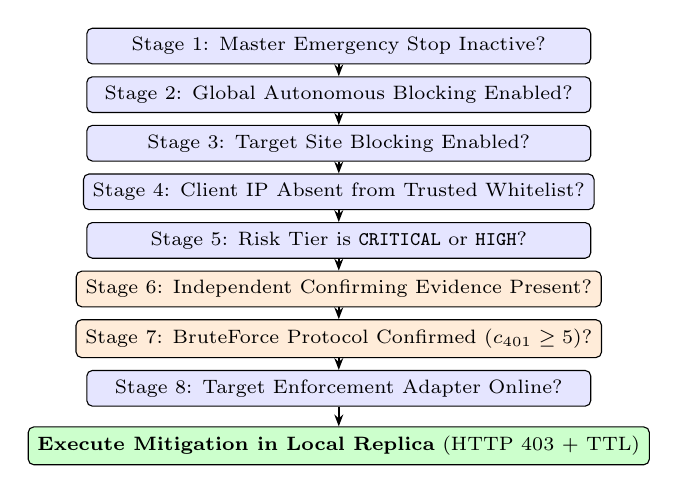
\begin{tikzpicture}[
    stepbox/.style={draw, rectangle, rounded corners=2pt, minimum width=6.4cm, minimum height=0.4cm, align=left, font=\scriptsize},
    arrow/.style={-{Stealth[length=1.5mm]}, thick}
]
    \node[stepbox, fill=blue!10] (s1) {Stage 1: Master Emergency Stop Inactive?};
    \node[stepbox, fill=blue!10, below=0.15cm of s1] (s2) {Stage 2: Global Autonomous Blocking Enabled?};
    \node[stepbox, fill=blue!10, below=0.15cm of s2] (s3) {Stage 3: Target Site Blocking Enabled?};
    \node[stepbox, fill=blue!10, below=0.15cm of s3] (s4) {Stage 4: Client IP Absent from Trusted Whitelist?};
    \node[stepbox, fill=blue!10, below=0.15cm of s4] (s5) {Stage 5: Risk Tier is \texttt{CRITICAL} or \texttt{HIGH}?};
    \node[stepbox, fill=orange!15, below=0.15cm of s5] (s6) {Stage 6: Independent Confirming Evidence Present?};
    \node[stepbox, fill=orange!15, below=0.15cm of s6] (s7) {Stage 7: BruteForce Protocol Confirmed ($c_{401} \ge 5$)?};
    \node[stepbox, fill=blue!10, below=0.15cm of s7] (s8) {Stage 8: Target Enforcement Adapter Online?};
    \node[stepbox, fill=green!20, below=0.25cm of s8, align=center] (block) {\textbf{Execute Mitigation in Local Replica} (HTTP 403 + TTL)};

    \draw[arrow] (s1) -- (s2);
    \draw[arrow] (s2) -- (s3);
    \draw[arrow] (s3) -- (s4);
    \draw[arrow] (s4) -- (s5);
    \draw[arrow] (s5) -- (s6);
    \draw[arrow] (s6) -- (s7);
    \draw[arrow] (s7) -- (s8);
    \draw[arrow] (s8) -- (block);
\end{tikzpicture}%
}
\caption{The 8-stage multi-factor enforcement verification rule chain governing automated closed-loop defense.}
\label{fig:rule_chain}
\end{figure}

Loopback boundary filters (\texttt{require\_local\_or\_admin}) restrict mutating endpoints to loopback origins (\texttt{127.0.0.1}), rejecting remote requests without administrative API keys.

% =========================================================================
% SECTION XIII: DISCUSSION AND OPERATIONAL CAVEATS
% =========================================================================
\section{Discussion, Operational Caveats, and Privacy Guarantees}
SentinelX implements zero payload inspection, discarding application-layer bytes and sanitizing URIs before queue insertion. 

\textit{Operational Caveats:} In reverse proxy or CDN environments, client IP correlation requires configuring upstream Nginx \texttt{realip} from trusted proxy subnets to prevent IP spoofing. Furthermore, temporal sliding-window correlation ($\pm 30\text{ s}$) requires NTP synchronization between flow exporters and web servers.

% =========================================================================
% SECTION XIV: CONCLUSION AND FUTURE WORK
% =========================================================================
\section{Conclusion and Future Work}
In this paper, we introduced \textbf{SentinelX-Shift}, an operational network intrusion detection and alert-prioritization architecture. Through an end-to-end audit of all eight partitions of CIC-IDS2017, we purged 594,712 duplicate vectors (21.03\%) and demonstrated the failure of shortcut learning. We established that unconstrained linear fusion collapses under zero-day distribution shifts, and introduced the Autoencoder-Anchored Gated Boost ($s_{\text{guard}}$) scoring function. Multi-seed LOFO benchmarks exposed the Zero-Day Generalization Deficit, resolved via Multi-Modal Protocol Guardrails requiring independent web/WAF corroboration. Our audited negative finding proved the unsuitability of post-hoc explanation stability as an automated gate. Finally, our dual-mode implementation achieved 1.25--2.45~ms CPU inference latency while enforcing strict Monitor-Only safety in production.

Future work will explore extending SentinelX to decentralized eBPF kernel probes for line-rate flow extraction, integrating privacy-preserving federated learning across multi-tenant SOCs, and developing transformer-based sequential representations for complex multi-stage attack scenarios.

% =========================================================================
% REFERENCES (Numerical Order of Appearance, Initials Preceding Last Name)
% =========================================================================
\begin{thebibliography}{37}

\bibitem{ring2019survey}
M.~Ring, S.~Wunderlich, D.~Scheuring, D.~Landes, and A.~Hotho, ``A survey of network-based intrusion detection data sets,'' \textit{Computers \& Security}, vol.~86, pp.~147--167, Sep.~2019.

\bibitem{chaabouni2019network}
N.~Chaabouni, M.~Mosbah, A.~Zemmari, C.~Sauvignac, and P.~Faruki, ``Network intrusion detection for IoT security based on machine learning: A review,'' \textit{IEEE Communications Surveys \& Tutorials}, vol.~21, no.~3, pp.~2671--2699, 3rd Quart., 2019.

\bibitem{apruzzese2023modeling}
G.~Apruzzese, M.~Andreolini, L.~Ferretti, M.~Marchetti, and M.~Colajanni, ``Modeling realistic adversaries in cybersecurity: A survey of recent literature,'' \textit{ACM Computing Surveys}, vol.~55, no.~7, pp.~1--37, Jul.~2023.

\bibitem{buczak2016survey}
A.~L.~Buczak and E.~Guven, ``A survey of data mining and machine learning methods for cyber security intrusion detection,'' \textit{IEEE Communications Surveys \& Tutorials}, vol.~18, no.~2, pp.~1153--1176, 2nd Quart., 2016.

\bibitem{sharafaldin2018toward}
I.~Sharafaldin, A.~H.~Lashkari, and A.~A.~Ghorbani, ``Toward generating a new intrusion detection dataset and intrusion traffic characterization,'' in \textit{Proc. 4th Int. Conf. Inf. Syst. Secur. Privacy (ICISSP)}, Funchal, Madeira, Portugal, 2018, pp.~108--116.

\bibitem{moustafa2015unsw}
N.~Moustafa and J.~Slay, ``UNSW-NB15: A comprehensive data set for network intrusion detection systems (UNSW-NB15 network data set),'' in \textit{Proc. IEEE Mil. Commun. Inf. Syst. Conf. (MilCIS)}, Canberra, ACT, Australia, 2015, pp.~1--6.

\bibitem{tavallaee2009detailed}
M.~Tavallaee, E.~Bagheri, W.~Lu, and A.~A.~Ghorbani, ``A detailed analysis of the KDD CUP 99 data set,'' in \textit{Proc. IEEE Symp. Comput. Intell. Cyber Secur. (CICS)}, Nashville, TN, USA, 2009, pp.~53--58.

\bibitem{sommer2010outside}
R.~Sommer and V.~Paxson, ``Outside the closed world: On using machine learning for network intrusion detection,'' in \textit{Proc. IEEE Symp. Secur. Privacy (S\&P)}, Oakland, CA, USA, 2010, pp.~305--316.

\bibitem{apruzzese2023role}
G.~Apruzzese, P.~Laskov, and A.~Schneider, ``The role of machine learning in cybersecurity: Hype vs. reality,'' \textit{IEEE Security \& Privacy}, vol.~21, no.~5, pp.~48--56, Sep.--Oct.~2023.

\bibitem{ardagna2023machine}
C.~Ardagna \textit{et al.}, ``Machine learning for cybersecurity: A comprehensive survey of challenges and future directions,'' \textit{IEEE Access}, vol.~11, pp.~45120--45145, May~2023.

\bibitem{arp2022dos}
D.~Arp, E.~Quiring, F.~Pendlebury, A.~Warnecke, F.~Pierazzi, C.~Wressnegger, R.~Cavallaro, and K.~Rieck, ``Dos and don'ts of machine learning in computer security,'' in \textit{Proc. 31st USENIX Secur. Symp.}, Boston, MA, USA, 2022, pp.~3971--3988.

\bibitem{geirhos2020shortcut}
R.~Geirhos \textit{et al.}, ``Shortcut learning in deep neural networks,'' \textit{Nature Machine Intelligence}, vol.~2, no.~11, pp.~665--673, Nov.~2020.

\bibitem{roesch1999snort}
M.~Roesch, ``Snort: Lightweight intrusion detection for networks,'' in \textit{Proc. 13th USENIX Conf. Syst. Admin. (LISA)}, Seattle, WA, USA, 1999, pp.~229--238.

\bibitem{claise2004cisco}
B.~Claise, G.~Sadasivan, V.~Valluri, and M.~Djernaes, ``Cisco Systems NetFlow Services Export Version 9,'' RFC 3954, Oct.~2004.

\bibitem{trammell2011introduction}
B.~Trammell and E.~Boschi, ``An introduction to the IP Flow Information Export (IPFIX) protocol,'' \textit{ACM SIGCOMM Comput. Commun. Rev.}, vol.~41, no.~1, pp.~66--72, Jan.~2011.

\bibitem{velan2015survey}
P.~Velan, M.~{\v{C}}erm{\'a}k, P.~{\v{C}}eleda, and K.~Dra{\v{s}}ar, ``A survey of methods for encrypted traffic classification and analysis,'' \textit{Int. J. Netw. Manag.}, vol.~25, no.~5, pp.~355--374, Sep.~2015.

\bibitem{sperotto2010overview}
A.~Sperotto, G.~Schaffrath, R.~Sadre, C.~Morariu, A.~Pras, and B.~Stiller, ``An overview of IP flow-based intrusion detection,'' \textit{IEEE Commun. Surveys Tuts.}, vol.~12, no.~3, pp.~343--356, 3rd Quart., 2010.

\bibitem{sultana2019survey}
N.~Sultana, N.~Chilamkurti, W.~Peng, and R.~Alhadad, ``Survey on SDN based network intrusion detection system using machine learning approaches,'' \textit{Peer-to-Peer Netw. Appl.}, vol.~12, no.~2, pp.~493--501, Mar.~2019.

\bibitem{ferrag2020deep}
M.~A.~Ferrag, L.~Maglaras, S.~Moschoyiannis, and H.~Janicke, ``Deep learning for cyber security intrusion detection: Approaches, datasets, and comparative study,'' \textit{J. Inf. Secur. Appl.}, vol.~50, p.~102419, Feb.~2020.

\bibitem{wang2017malware}
W.~Wang, M.~Zhu, X.~Zeng, X.~Wang, and J.~Yang, ``Malware traffic classification using convolutional neural network for representation learning,'' in \textit{Proc. Int. Conf. Inf. Netw. (ICOIN)}, Da Nang, Vietnam, 2017, pp.~712--717.

\bibitem{mirsky2018kitsune}
Y.~Mirsky, T.~Doitshman, Y.~Elovici, and A.~Shabtai, ``Kitsune: An ensemble of autoencoders for online network intrusion detection,'' in \textit{Proc. Netw. Distrib. Syst. Secur. Symp. (NDSS)}, San Diego, CA, USA, 2018, pp.~1--15.

\bibitem{zhou2017anomaly}
C.~Zhou and R.~C.~Paffenroth, ``Anomaly detection with robust deep autoencoders,'' in \textit{Proc. 23rd ACM SIGKDD Int. Conf. Knowl. Discovery Data Mining}, Halifax, NS, Canada, 2017, pp.~665--674.

\bibitem{haas2020aggressiveness}
S.~Haas and R.~Fischer, ``On the aggressiveness of CIC-IDS2017: Pitfalls and improvements,'' in \textit{Proc. 15th Int. Conf. Availability, Rel. Secur. (ARES)}, Virtual Event, 2020, pp.~1--10.

\bibitem{engelen2021troubleshooting}
G.~Engelen, V.~Rimmer, and W.~Joosen, ``Troubleshooting an incomplete machine learning pipeline in network intrusion detection,'' in \textit{Proc. 43rd ACM Workshop Artif. Intell. Secur. (AISEC)}, Virtual Event, 2021, pp.~107--118.

\bibitem{panigrahi2018detailed}
R.~Panigrahi and S.~Borah, ``A detailed analysis of CICIDS2017 dataset for designing network intrusion detection systems,'' \textit{Int. J. Eng. Technol.}, vol.~7, no.~3.24, pp.~479--482, 2018.

\bibitem{rosay2020improving}
A.~Rosay, F.~Carlier, and E.~Renault, ``Improving network intrusion detection systems through feature selection and dataset enhancement,'' in \textit{Proc. IEEE 45th Conf. Local Comput. Netw. (LCN)}, Sydney, NSW, Australia, 2020, pp.~445--448.

\bibitem{lashkari2017characterization}
A.~H.~Lashkari, G.~D.~Gil, M.~S.~I.~Mamun, and A.~A.~Ghorbani, ``Characterization of tor traffic using time based features,'' in \textit{Proc. 3rd Int. Conf. Inf. Syst. Secur. Privacy (ICISSP)}, Porto, Portugal, 2017, pp.~253--262.

\bibitem{thorne2023evaluating}
J.~Thorne, G.~Apruzzese, and M.~Colajanni, ``Evaluating machine learning for network intrusion detection: A systematic review of datasets and validation strategies,'' \textit{Computers \& Security}, vol.~128, p.~103140, May~2023.

\bibitem{verkerken2022towards}
T.~Verkerken, L.~D'hooge, T.~Wauters, B.~Volckaert, and F.~De~Turck, ``Towards realistic evaluation of machine learning for network intrusion detection: Leave-one-attack-out validation,'' \textit{IEEE Access}, vol.~10, pp.~78450--78465, Jul.~2022.

\bibitem{nwakanma2023generalization}
C.~I.~Nwakanma \textit{et al.}, ``Generalization bounds and out-of-distribution evaluation for machine learning in zero-day network security,'' \textit{IEEE Trans. Inf. Forensics Security}, vol.~18, pp.~3125--3139, Jun.~2023.

\bibitem{lundberg2017unified}
S.~M.~Lundberg and S.-I.~Lee, ``A unified approach to interpreting model predictions,'' in \textit{Proc. 31st Conf. Neural Inf. Process. Syst. (NeurIPS)}, Long Beach, CA, USA, 2017, pp.~4765--4774.

\bibitem{ribeiro2016why}
M.~T.~Ribeiro, S.~Singh, and C.~Guestrin, ``Why should I trust you?: Explaining the predictions of any classifier,'' in \textit{Proc. 22nd ACM SIGKDD Int. Conf. Knowl. Discovery Data Mining}, San Francisco, CA, USA, 2016, pp.~1135--1144.

\bibitem{wang2020explainable}
M.~Wang, K.~Zheng, Y.~Yang, and X.~Wang, ``An explainable machine learning framework for network intrusion detection systems,'' \textit{IEEE Access}, vol.~8, pp.~73127--73141, Apr.~2020.

\bibitem{noor2023xai}
F.~Noor, M.~A.~Khan, and S.~U.~Rehman, ``XAI-NIDS: Explainable artificial intelligence for network intrusion detection systems,'' \textit{IEEE Trans. Netw. Serv. Manag.}, vol.~20, no.~3, pp.~2450--2463, Sep.~2023.

\bibitem{mishra2022robustness}
P.~Mishra \textit{et al.}, ``On the robustness of feature attribution methods in adversarial cyber security environments,'' in \textit{Proc. IEEE Eur. Symp. Secur. Privacy Workshops (EuroS\&PW)}, Genoa, Italy, 2022, pp.~110--121.

\bibitem{alvarez2018robustness}
D.~Alvarez-Melis and T.~S.~Jaakkola, ``On the robustness of interpretability methods,'' in \textit{Proc. ICML Workshop Human Interpretability Mach. Learn. (WHI)}, Stockholm, Sweden, 2018, pp.~1--9.

\bibitem{corona2013adversarial}
I.~Corona, G.~Giacinto, and F.~Roli, ``Adversarial attacks against machine learning-based network intrusion detection systems: A survey,'' \textit{Computers \& Security}, vol.~38, pp.~119--132, Oct.~2013.

\end{thebibliography}

\end{document}
